%Notes on SSD with Multiscale Feature Fusion
%Available at https://www.mdpi.com/2072-4292/11/5/594/htm

This paper presents a novel architecture along with a new loss system, allowing for more precise bounding boxes along detected objects. The new architectures incorporates ideas similar to YOLT\cite{yolt} where multiple detectors are trained and ran at different scales. This time the different scales detection is directly incorporated into the architecture itself: the feature maps from different layers are concatenated together. This approach allows the model to fully use the low level feature map with high resolution along with the high level feature maps incorporating more semantic information.

The model is trained and tested on two different datasets: the RSD-GOD dataset, a new dataset comprising of 5 different categories and 18K annotated images introduced by this paper, and the NWPU VHR-10\cite{nwpu} dataset.

\subsection{Architecture}
\subsubsection{Base Feature Extractor}
The proposed network is heavily based on the Darknet-53 architecture and reuses most of it features. 53 Convolutional layers are used, without pooling layers. The network reduce the features dimension by 2 by applying a stride. The Network also uses residual blocks containing $1 \times 1$ and $3 \times 3$ convolutional filters and 23 residual blocks. Batch normalisation\cite{batchNorm} instead of dropout is used to control overfitting and convergence during training. The network uses leaky ReLU activations on all convolutional layers. 

\begin{figure}[h!]
	\centering
	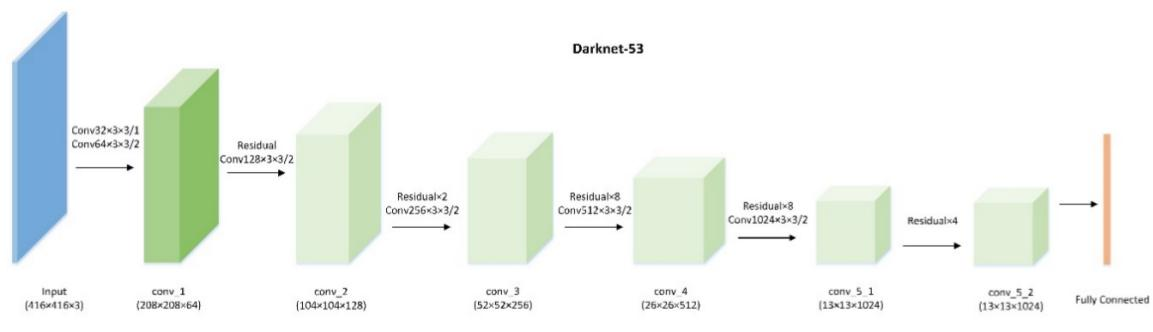
\includegraphics[width=\textwidth]{darknetArchi.jpg}
	\caption[Architecture of the Darknet 53, used as a base network for features extraction in the Single-Shot Object Detection Framework]{Architecture of the Darknet 53, used as a base network for feature extraction}
	\label{}
\end{figure}

\subsubsection{Multi-scale feature fusion detector}
To allow the detector to fully exploit both low level high resolution with fine detail feature maps and high level semantic features, multi-scale feature are used. 

\begin{figure}[h!]
	\centering
	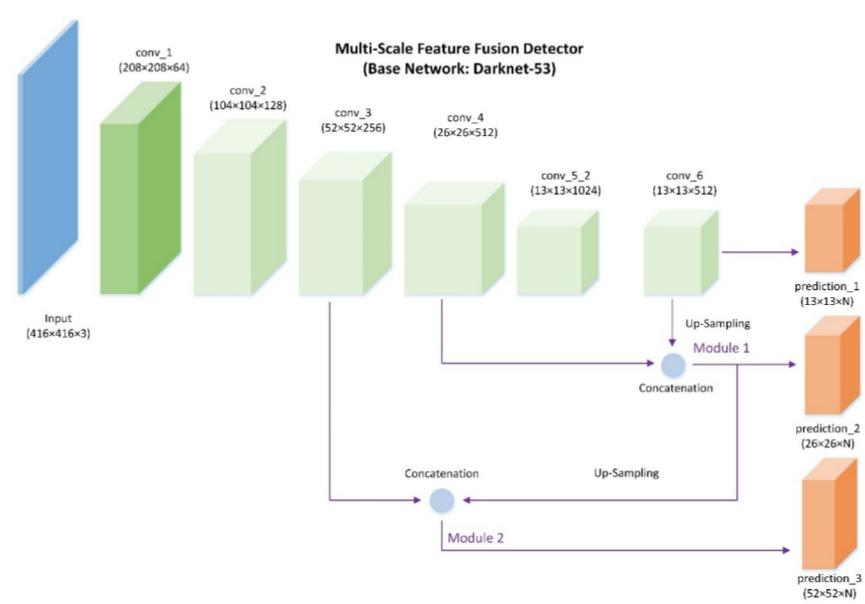
\includegraphics[width=\textwidth]{msFusionDetectorArchi.jpg}
	\caption[]{General architecture of the multi-scale feature fusion detector. The model uses Darknet-53 as the base feature extractor. Three predictions are generated at three different scales.}
	\label{}
\end{figure}

Three convolutional layers at different scales of the base feature extractor are used to make predictions. The first-scale predictions are made using an added convolutional layer on top of the last convolutional layer of the base feature detector. Following the article definitions, we will call this convolutional prediction layer \verb|conv_6|. Two feature fusion modules are used to combine shallow feature. The first fusion module takes the prediction of the \verb|conv_6| layer, upsamples it and concatenate it to the feature maps yielded by the \verb|conv_4| layer. This gives out the second scale predictions. Finally, the second fusion modules takes the feature maps of the \verb|conv_3| layer and concatenate it to the output of the first fusion modules, after up-sampling. This yield the third and final prediction. 

\subsubsection{Multi-scale feature fusion module}
Three multi-scale feature fusion module are used to create 3 different scale prediction. 

\begin{figure}
	\centering
	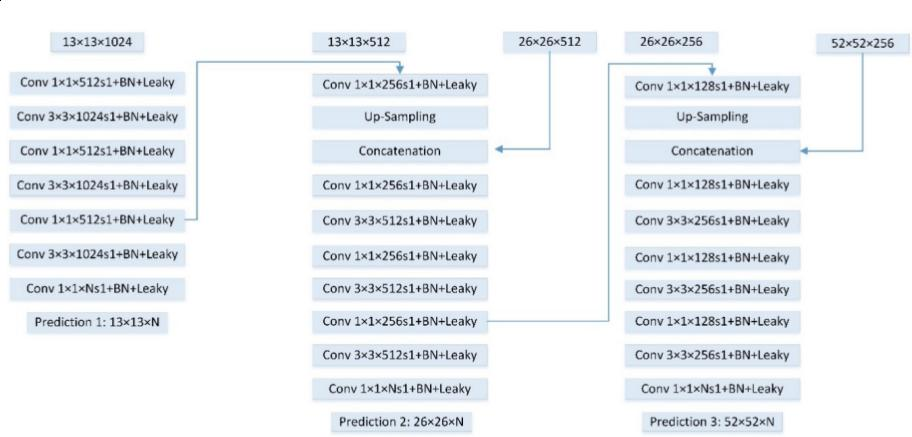
\includegraphics[width=\textwidth]{msFeatureFusionModule.jpg}
	\caption[]{Multi-scale feature fusion module. The Feature maps from different layers are merged through up-sampling and concatenation. Each convolutional layer is batch-normalized, uses leaky ReLU activations, and have a stride of 1.}
	\label{fig:multiScaleFusionModule}
\end{figure}

In a multi-scale feature fusion module, the dimension of the input feature maps are first reduced through the use of $1 \times 1$ convolutional kernel. High level feature maps are up-sampled after the $1 \times 1$ convolution to be same size as the lower level feature maps. Then, the high level feature maps are concatenated with the lower level feature maps. Alternate $1 \times 1$ and $3 \times 3$ convolutional layer are then used to progressively reduce the dimensions of the feature maps and make predictions. Figure~\ref{fig:multiScaleFusionModule} show details of the feature fusion module.

\subsubsection{Anchors and predictions}
Since the model is unstable during early training iterations, anchors are used, similar to the ones used in Faster R-CNN~\cite{FasterRCNN}. The designed network outputs three kind of feature maps with different size : $13 \times 13$, $26 \times 26$, $52 \times 52$. $B$ anchors are generated and the corresponding B bounding boxes are predicted for each grid cell. During the training, the network outputs 5 coordinate values $t_x, t_y, t_w, t_h, t_o$; the final location of the predicted bounding box is obtained through the anchor size and the network outputs. 

The location of the center of the bounding boxes ($b_x, b_y$) is relative to the grid cell offset ($c_x, c_y$) and the sigmoid activation function value of the location coordinates ($t_x, t_y$). Here ($c_x, c_y$) denotes the offsets from the top left corner of the original image to the current grid cell. The width and height of anchors are denoted as ($p_w, p_h$). $p_o$ denotes the confidence score of object probability. The $\sigma$ denotes the sigmoid function. Applying the sigmoid function on the predicted $t_x, t_y, t_o$ normalize their value and stabilize the model during training.

We compute $b_x, b_y, b_w, b_h$ and $p_o$ using the following formulas:

\begin{equation}
	b_x = \sigma(t_x) + c_x
\end{equation}

\begin{equation}
	b_y = \sigma(t_y) + c_y
\end{equation}

\begin{equation}
	b_w =  p_w e^{t_w}
\end{equation}

\begin{equation}
	b_h =  p_h e^{t_h}
\end{equation}

\begin{equation}
	p_o = \sigma(t_o)
\end{equation}

For each predictions module, 3 anchor priors with different scales are used ($B= 3$). K-means clustering have been applied on the annotated bounding boxes in the training data in order to obtain suitable priors.

The network outputs four coordinates, one object confidence information and C class probabilities for each bounding box. The dimension of the network output tensor is then $S \times S \times N$, where $S$ is the grid size, and $N = (5 + C) \times B$

\begin{figure}
  \centering
  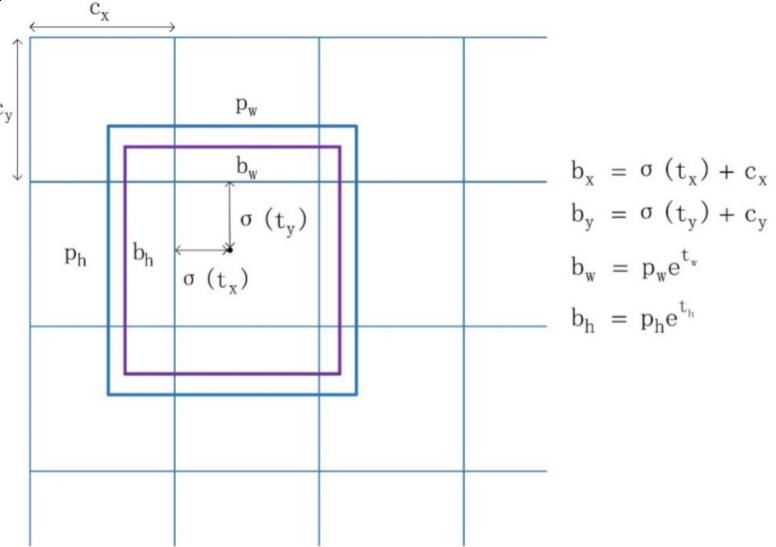
\includegraphics[width=\textwidth]{anchors.jpg}
	\caption[Anchors and location predictions]{The model generates 4 coordinates: $t_x, t_y, t_w$ and $t_h$. The center location of the final bounding box $(b_x, b_y)$ is relative to the grid cell offsets $(c_x, c_y)$ and the sigmoid activation function value of location coordinates $(t_x, t_y)$. $(c_x, c_y)$ denotes the offsets from the top left corner of the original image to the current grid cell}
  \label{}
\end{figure}
\subsubsection{Loss Function}
The training objective loss is defined as the sum of a localization loss ($L_{loc}$), a confidence loss ($L_{conf}$) and a classification loss ($L_{cla}$). 

The localization and confidence are computed using the squared error loss (see equations~\ref{eq:lossLoc} and~\ref{eq:lossConf}). The class loss is computed using the categorical crossentropy loss and is given in equation~\ref{eq:lossClass}.

\begin{equation}
	L_{overall} = L_{loc} + L_{conf} + L_{cla}
\end{equation}

\begin{equation}\label{eq:lossLoc}
	L_{loc} = \lambda_{coord} \sum_{i=0}^{S^2} \sum_{j=0}^B [(x_i \hat{x_i})^2 + (y_i - \hat{y_i})^2 + (w_i - \hat{w_i})^2 + (h_i - \hat{h_i})^2]
\end{equation}

\begin{equation}\label{eq:lossConf}
	L_{conf} = \lambda_{obj}  \sum_{i=0}^{S^2} \sum_{j=0}^B P^{obj} (c_i - \hat{c_i})^2 + \lambda_{noobj} \sum_{i=0}^{S^2} \sum_{j=0}^B (1 - P^{obj}) (c_i - \hat{c_i})^2   
\end{equation}

\begin{equation}\label{eq:lossClass}
	L_{cla} = -\lambda_{cla} \sum_{i=0}^{S^2} P^{obj} log(\hat{p_i})
\end{equation}

Here, $\lambda_{coord}, \lambda_{noobj}$ and $\lambda_{cla}$ represents scaling factors for the weight localization loss, the confidence loss and classification loss. $P^{obj}$ is probability that there is an object in the box. Predicted bounding boxes without objects are more penalized. 

The authors used the following values of $\lambda$: $\lambda_{coord} = 1, \lambda_{obj} = 5, \lambda_{noobj} = 1, \lambda_{cla} = 1$
\subsubsection{Soft Non-Maximum Suppression}

The proposed detection method generates a large number of cluttered bounding boxes. In traditional one stage detection pipelines, Non Maximum Suppression (NMS) is used to remove repetitive bounding boxes. NMS ranks location candidates according to their classification, and removes overlapping bounding boxes with the lowest scores. 

Here, this method might cause the framework to miss part of neighboring detections, whose classification scores are lower. Instead of removing the location candidates, the Soft Non Maximal Suppression assign a new classification score to the bounding boxes, following equation~\ref{eq:snms}

\begin{equation}\label{eq:snms}
	s_i =
	      \begin{cases}
		      s_i & iou(b_i, b_M) < T; i \neq M\\
		      s_i * f(iou(b_i, b_M)) & iou(b_i, b_M) \geq T; i \neq M\\
	      \end{cases}  
\end{equation}

Where $b_i$ denotes the $i$th bounding box in the location candidates and $b_M$ is the bounding box with the maximum score. If the IoU between $b_i$ and $b_M$ is larger than a specified threshold $T$, a decayed score will be given to $b_i$ using the Gaussian penalty function:

\begin{equation}
	f(iou(b_i, b_M) = exp[\frac{-(iou(b_i, b_M))^2}{\rho}]
\end{equation}

\subsection{Results}
The authors tested their method on the RSD-GOD dataset and compared it to other detection framework: Faster R-CNN\cite{FasterRCNN}, SSD\cite{ssd}, YOLO2\cite{yolov9000}. The authors also tested their method with and without the Soft-NMS. The table with results are fairly large, and so are replicated in the appendices. Results for the RSD-GOD datasets are shown in table\ref{tab:SSDres}.

Faster R-CNN obtains the best precision score for the airport class. However, the proposed methods with the soft-NMS obtain the best score for all other classes. 
The detector was also trained and tested on the NWPU VHR-10\cite{nwpu} dataset, along with a collection of part detectors (COPD)\cite{copd}, rotation-invariant CNN (RICNN)\cite{ricnn} and a R-P-Faster R-CNN\cite{rpfrcnn} and the detectors used for the evaluation of RSD-GOD. COPD and RICNN are rotation-invariant frameworks with SVM classifier for geospatial object detection. COPD uses hand-crafted features while RICNN applies learned features from the CNN.

As can be seen in table \ref{tab:SSDresNWPU}, SSD obtains the best precision score for the airplane and ship class, along with the baseball diamond. Faster R-CNN obtains the best score for basketball court and YOLOv2 the best score for ground track field. For all other classes, the proposed method with soft-NMS obtains the best score.

\begin{table}[h!]
	\centering
	\begin{tabular}{@{}llllllll@{}}
		\toprule
		Methods                  & COPD  & R-P-Faster R-CNN & RICNN & SSD    & Faster R-CNN & YOLO2     & Proposed   \\ \midrule
		Backbone                 & -     & VGG16            & -     & VGG-16 & ResNet50     & Darknet50 & Darknet-53 \\
		Average Running Time (s) & 1.070 & 0.150            & 8.770 & 0.027  & 0.430        & 0.026     & 0.057      \\ \bottomrule
	\end{tabular}
	\caption{Average running time of the tested methods}
	\label{tab:perf}
\end{table}
